\section{DHCP Setup}
This section describes how the \textbf{DHCP service} was set up in the \textit{Internal router} machine, the one reachable at address \textbf{100.100.2.1}.\\
The router was accessed via web browser in the \textbf{Kali machine} (\textbf{100.100.2.100} as static IP address) through the given credentials, and then the desired service was configured through the \textbf{OPNSense} administration panel.\\
The following steps were taken to give the service the proper configuration provided by the assignment:\\

\begin{itemize}
\item the service was enabled on the router, as pictured in \textbf{Figure 2}, with the option \textbf{"Deny unknown clients"} checked in order to prevent undesired clients (the ones with a MAC address that is different from the ones specified and thus without ARP entries registered) from obtaining a dynamic IP address in the network. Keep also in mind that the subnet mask was already specified in the \textbf{CLIENTS} interface for the router, and the same goes for other services - such as \textbf{Unbound DNS}, so that these settings were not required to be configured again;
\item the address range was initially specified as \textbf{100.100.2.101 - 100.100.2.253} so to avoid a re-assignment of known static IP addresses in the network - that is to say, those belonging to the Kali machine, the Arpwatch machine and, of course, the router itself. Later on, as pictured in \textbf{Figure 3}, a new pool of addresses was specified in the range \textbf{100.100.2.2 - 100.100.2.99} so to comprehend all the addresses that are not known to be assigned in the network;
\item as pictured in \textbf{Figure 4}, the partial \textbf{MAC addresses} pointed out in the assignment as allowed to make use of the service were specified in the configuration, so that the only machines able to receive DHCP offers from the router will be the ones exhibiting these MAC addresses;
\item as pictured in \textbf{Figure 5}, the six desired MAC addresses were then specified in the \textbf{DHCP Static Mappings} and a \textbf{Static ARP entry} was created for each of them so to remember their MAC address and mark them as known clients.
\end{itemize}

\begin{figure}[H]
\centering
\begin{minipage}{.5\textwidth}
  \centering
  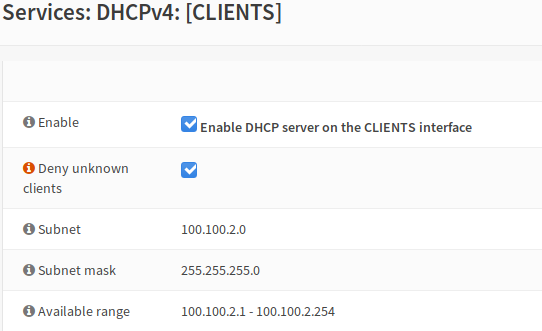
\includegraphics[width=1\textwidth]{dhcp_clients.png}
  \caption[a]{Enabling the DHCP service.}\label{fig:2}
\end{minipage}%
\begin{minipage}{.5\textwidth}
  \centering
  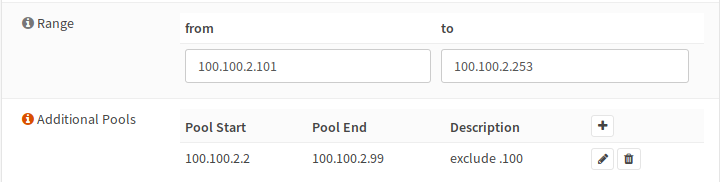
\includegraphics[width=1\textwidth]{dhcp_range.png}
  \caption[a]{Range of assignable addresses.}\label{fig:3}
\end{minipage}
\end{figure}

\begin{figure}[H]
\centering
\begin{minipage}{.5\textwidth}
  \centering
  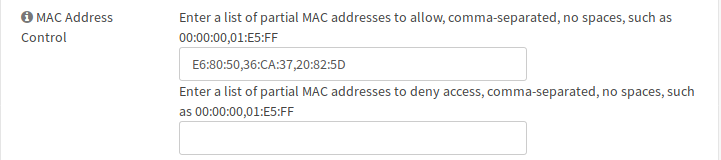
\includegraphics[width=1\textwidth]{dhcp_mac_rules.png}
  \caption[a]{The partial MAC addresses specified.}\label{fig:4}
\end{minipage}%
\begin{minipage}{.5\textwidth}
  \centering
  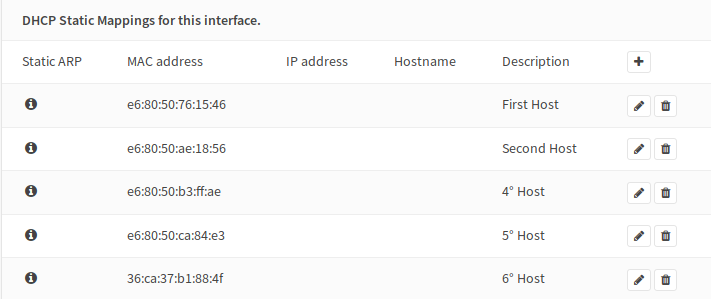
\includegraphics[width=1\textwidth]{dhcp_static_mappings.png}
  \caption[a]{DHCP Static Mappings for the desired addresses - one is missing due to screen resolution on openVNC.}\label{fig:5}
\end{minipage}
\end{figure}

Once the \textbf{DHCP service} was confirmed running on the router, it was tested directly from the \textbf{Kali machine} by deleting the IP address set by default on \textbf{eth0} and thus trying to obtain a new one through the \textbf{DHCP service} of the router. First, as pictured in \textbf{Figure 6}, the \textbf{dhclient} command was run so that the machine could obtain a new dynamic IP address on the interface \textbf{eth0} - the machine has by default a \textbf{MAC address} on interface \textbf{eth0} which falls under the allowed addresses specified in the configuration. A \textbf{DHCP offer} was received by the router, and a new IP address was obtained, positively assessing the functioning of the service so far.\\
Again from the \textbf{Kali machine}, the \textbf{MAC address} of \textbf{eth0} was then changed to one that should not be allowed to request a new IP to the service, as pictured in \textbf{Figure 7}. The \textbf{dhclient} command was run again, and this time no offer was received, thus confirming that the service is only leasing IP addresses to machines having the desired \textbf{MAC addresses} on their interfaces. Since the machine had already received a lease by the service in the previous step, though, it was able to re-use the one previously obtained, but if it hadn't then no IP address would have been obtained.\\
Same test was run by slightly changing the original \textbf{MAC address} maintaining the first three bytes (\textbf{e6:80:50}), so to obtain a partial match of the address; as we can see from \textbf{Figure 8}, again no DHCP offer was received, confirming the desired behavior of the service.

\begin{figure}[H]
\centering
\begin{minipage}{.33\textwidth}
  \centering
  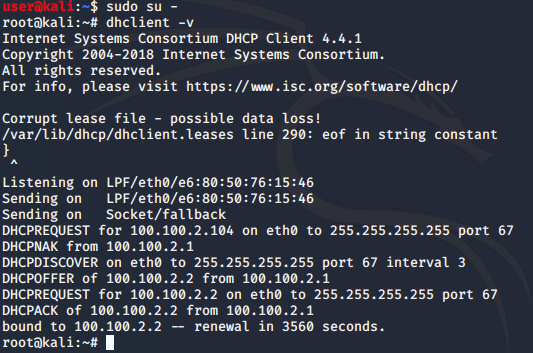
\includegraphics[width=1\textwidth]{dhcp_kali_macOk.png}
  \caption[a]{Kali machine with right MAC address on eth0 receiving a new IP address.}\label{fig:6}
\end{minipage}%
\begin{minipage}{.33\textwidth}
  \centering
  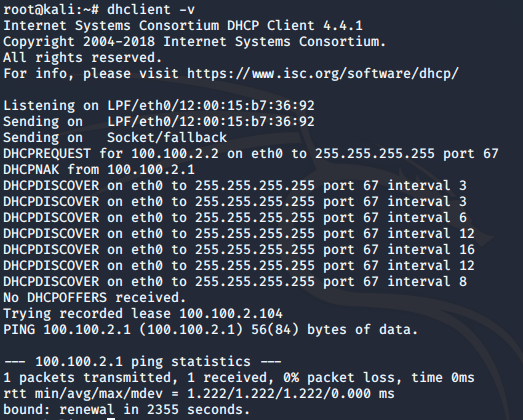
\includegraphics[width=1\textwidth]{dhcp_kali_macNotOk.png}
  \caption[a]{Kali machine unable to receive a DHCP offer due to its modified MAC address.}\label{fig:7}
\end{minipage}
\begin{minipage}{.33\textwidth}
  \centering
  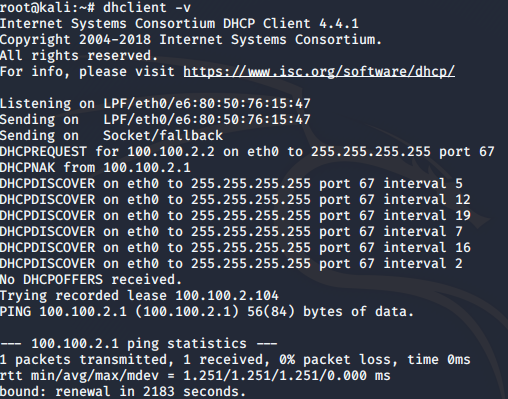
\includegraphics[width=1\textwidth]{dhcp_kali_macNotOk2.png}
  \caption[a]{Kali machine unable to receive a DHCP offer due to its slightly modified MAC address.}\label{fig:8}
\end{minipage}
\end{figure}
